\documentclass[11pt,a4paper]{article}
\usepackage[margin=22mm]{geometry}
\usepackage{fontspec,xeCJK,amsmath,amssymb,booktabs,graphicx,hyperref,fancyhdr,longtable,array,xcolor}
\setmainfont[Path=/home/qiuyong/fonts/,BoldFont=ARIALBD.TTF,ItalicFont=ARIALI.TTF]{arial.ttf}
\setCJKmainfont[Path=/home/qiuyong/fonts/]{1611458310630572.ttf}
\hypersetup{colorlinks=true,urlcolor=blue,linkcolor=blue}\pagestyle{fancy}\fancyhf{}
\fancyhead[L]{六分子关联泛函：本周归档与采样预算}\fancyfoot[C]{\thepage}\setlength{\headheight}{15pt}\setlength{\parskip}{5pt}\setlength{\emergencystretch}{4em}
\graphicspath{{docs/reports/WEEKLY_CDFT_DATA_20261028/figures/}}
\begin{document}
\begin{center}{\LARGE 六分子关联泛函的数据准备}\\[7pt]
{\large 本周证据归档、可编辑流程与采样预算}\\[5pt]
2026-10-22 至 2026-10-28\end{center}

\noindent\textbf{研究问题。} 以水、氨、甲烷、乙烯、乙烷和二氧化碳为对象，能否先通过机器学习势与可核查的统计采样获得密度及两体关联，再训练一个对分子与状态变化有泛化能力的 $c_1/c_2$ 模型？本文将本周两个仓库的准备工作和后续预算放在同一条路径中。文献各自的采样单位不同，本报告先算基础轨迹与目标验证，再列状态覆盖缺口。

\textbf{目前可支持的判断。} 六分子教师单点和学生势的留出集误差有记录；OFF23 水轨迹已有逐帧目标能量与权重诊断。它们证明可做数据管道探索，但尚未证明六种分子的目标体系密度、$g(r)$、$c_1$ 或 $c_2$ 已达训练标签质量。尤其只有一条 300 K、384 水分子的 OFF23 长轨迹；没有与其对应的独立 POLAR 长轨迹。

\textbf{本报告建议。} 先为六种分子建立基础源轨迹；在目标能量、重叠和误差允许的范围内，温度及外场通过后处理复用同一批构型。先做独立副本与教师验证，再按缺口补密度锚点。后文 $1\,\mathrm{ns}$ 是\emph{预算情景}，不是独立样本数或已完成计算。

\textbf{版本。} 本次证据快照：\href{https://github.com/Yong-Q/test/tree/65a0423}{test 65a0423}，\href{https://github.com/Yong-Q/symmetrix-polar/tree/68f08d1}{symmetrix-polar 68f08d1}。后续仓库变更需重新核对对应证据。所有图的数值源及脚本随归档保存。

\section{科学背景：从密度与关联到泛函}
\subsection{PNAS：带外场的密度用于学习 $c_1$}
Bui 与 Cox 将不同流体和相互作用势下的随机外场 MD 密度用于训练一体直接关联泛函。原文使用单独的流体／势模型，而不是已经得到跨分子的统一泛函。其水与二氧化碳例子使用已有机器学习势，在平面随机外势下生成密度；每个流体和势的训练数据约 500--1000 个独立模拟，生产时间至少 $1\,\mathrm{ns}$，时间步长 $0.5\,\mathrm{fs}$。外力施加在定义的分子中心位点，化学势作为每次模拟的潜变量学习［1，材料与方法］。

对应平衡关系可写成
\begin{equation}
c_1(z;[\rho],T)=\ln[\rho(z)\Lambda^3]+\beta V_{\rm ext}(z)-\beta\mu,\qquad \beta=(k_BT)^{-1}.
\end{equation}
因此只统计密度尚不能无条件给出绝对 $c_1$；还需外场、温度、化学势与理想参考。固定 $N$ 的 MD 可以采用与 PNAS 一致的潜变量策略，但要明确密度变量、有限尺寸和参考基准。

\subsection{PRL：体相关联监督 $F_{\rm ex}$ 的二阶导数}
Dijkman 等在均匀 Lennard--Jones 体相中用 GCMC 采样 $g(r)$，通过 OZ 方程得到体相 $c_2$，训练自由能网络的 Hessian；该分支并非将每个外场的 $c_1$ 真值直接作为监督。其对照模型则使用非均匀密度对应的一阶导数数据［2］。
\begin{equation}
h(r)=g(r)-1,\quad S(k)=1+\rho_b\hat h(k),\quad
\hat c_2(k)=\frac{\hat h(k)}{1+\rho_b\hat h(k)}.
\end{equation}
式子适用于均匀、各向同性、单组分且定义相匹配的标量密度。水的氧位点与分子质心是不同变量；取向分辨或不均匀体系需对应的多分量／位置依赖关系。原文为 Lennard--Jones 模型而非本项目六分子的精度认证。

\subsection{JCTC：显式位置--取向密度}
Yang 等研究超临界 CO$_2$，以单方向位置及两个取向角描述分子密度，并使用取向相关的 $c_1$ 神经算子；这与本周主要做的分子质心密度不同。其 GCMC 支持信息记载单次模拟约 $4\times10^6$ 个试探步平衡、$5\times10^7$ 个试探步生产；主文采用8个温度和10个化学势条件，支持信息描述给定外场下320组密度剖面［7］。这些 MC 试探步、MD 轨迹帧与独立剖面不能混算。六分子包含水等非线性分子时，取向变量及对称性也需要重新定义。

\subsection{文献数量与本工作预算的关系}
PNAS 的每流体／势500--1000个外场模拟，是独立生成数据的论文设置；PRL 的800个体相密度--关联训练样本来自 Lennard--Jones 体相 GCMC；JCTC 的320组剖面来自其 CO$_2$ GCMC 设置。它们对应不同的体系、温度、采样和标签，并不要求本项目无条件重做同数目的模拟。本报告先探索\textbf{复用基础轨迹}，但需以目标观测量的误差与重叠证据确认实际能复用多少条件。

\section{整体研究流程及当前状态}
图1从已核对的文献和六分子教师数据出发，将势函数、采样、标签、统一模型及物理性质贯通。\textcolor{black}{红色节点表示待完成或未验证}；黄色节点表示已有局部结果但尚不足以支持下一层结论。PDF 是可阅读的静态视图；同目录 HTML 可拖动节点、修改文字和状态，导出 JSON 或 SVG。
\begin{figure}[htbp]\centering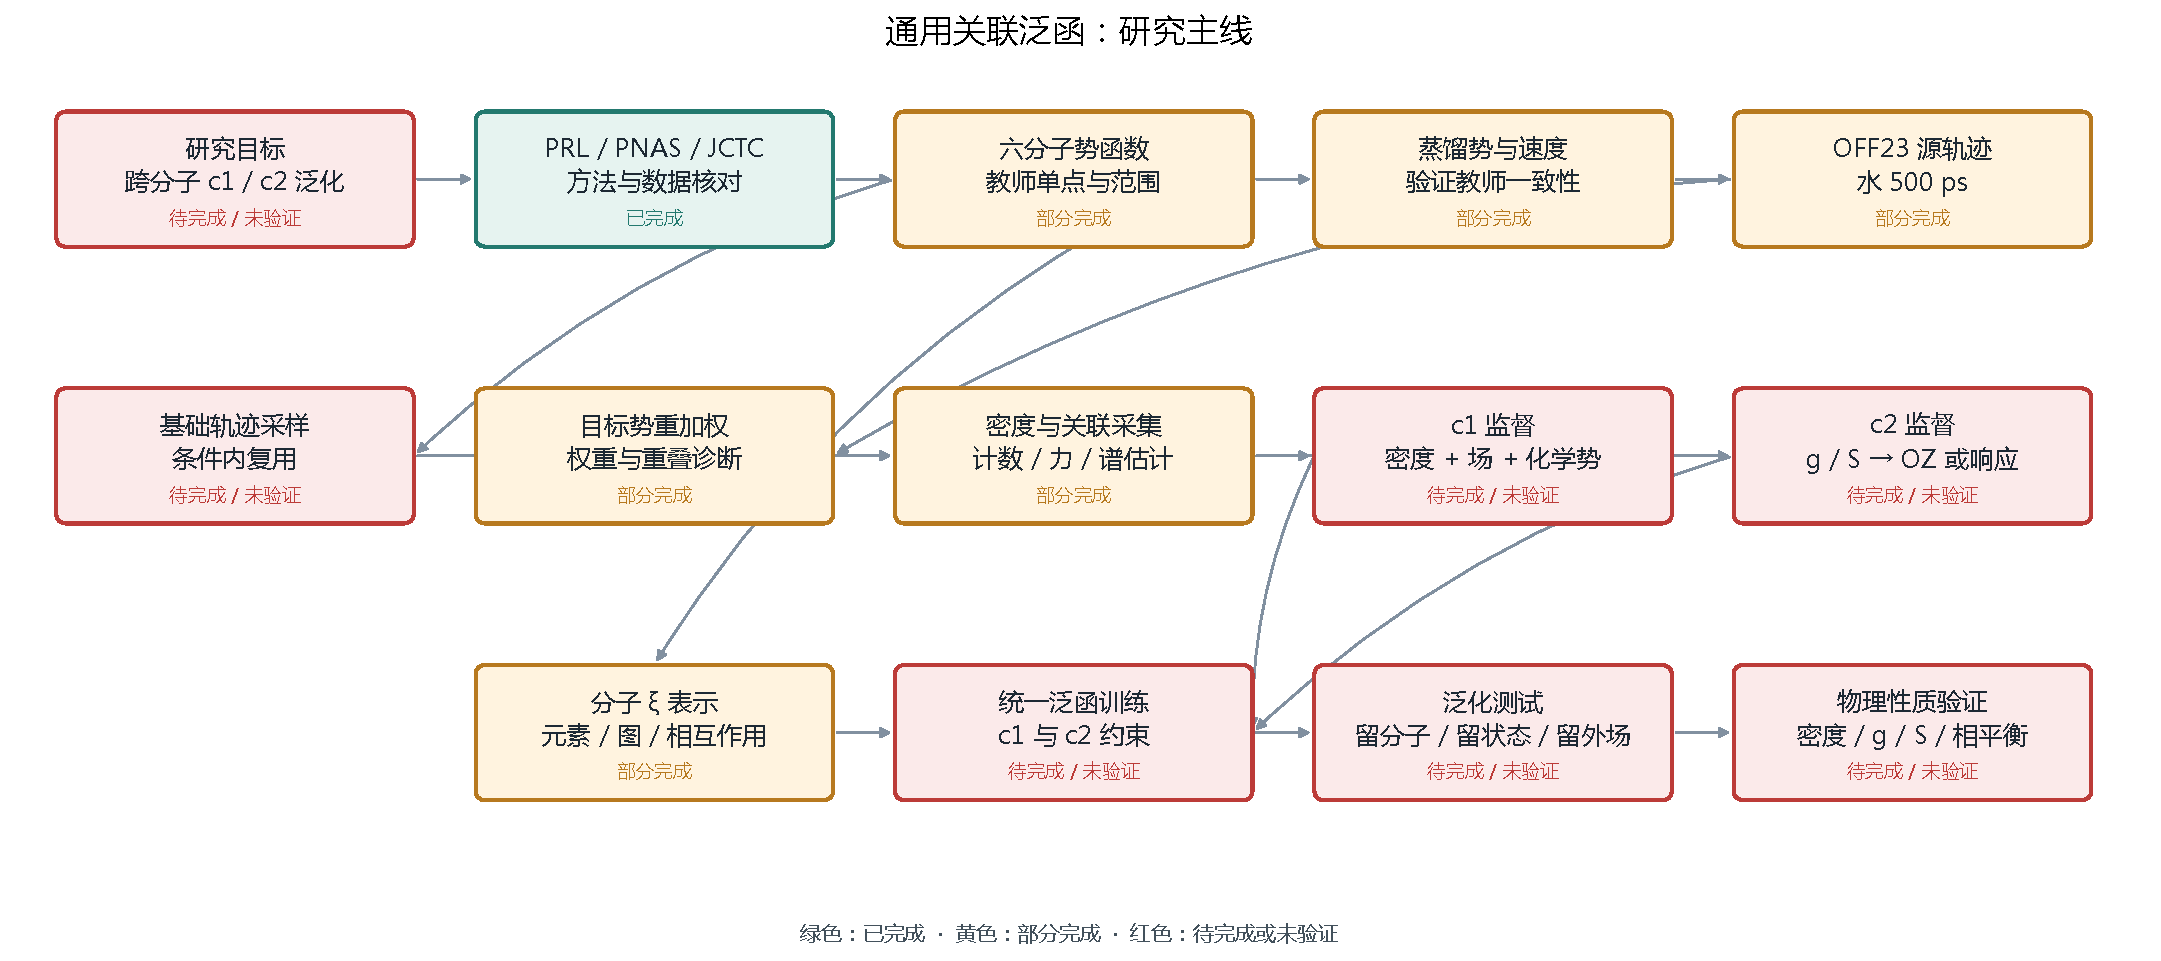
\includegraphics[width=\textwidth]{01_research_flow.pdf}
\caption{六分子数据到关联泛函的研究流程。节点颜色是截至本次归档的状态，不代表永久定论；输入、输出与尚缺证据见在线工作台节点说明。}\end{figure}

\section{本周结果：势函数与重加权}
\subsection{六分子教师与学生}
六分子教师烟测覆盖 H$_2$O、NH$_3$、CH$_4$、C$_2$H$_4$、C$_2$H$_6$ 和 CO$_2$，每种8个构型、每盒12个分子。随机构型有不合理近接，CO$_2$ 最大力约 $37.5\,\mathrm{eV}/\text{\AA}$，故只能证明单点与写出流程可运行，不能当作平衡结构集［3］。

Plan D 的已有留出集对教师能量/力结果由源 JSON 汇总，图2分别画出六种分子的体相子集。总留出集为 3465 帧、总能量 MAE 约 $1.12\,\mathrm{meV/atom}$、力分量 MAE 约 $7.75\,\mathrm{meV}/\text{\AA}$；样本由不同状态混合，不能将其误认成独立实验误差。CO$_2$ 体相力误差最大，约 $23.62\,\mathrm{meV}/\text{\AA}$。电荷／偶极头的已有评价和主干 E/F 评价涉及不同数据与功能，尚需完整力场耦合、外场、动力学稳定性和外推验证。
\begin{figure}[htbp]\centering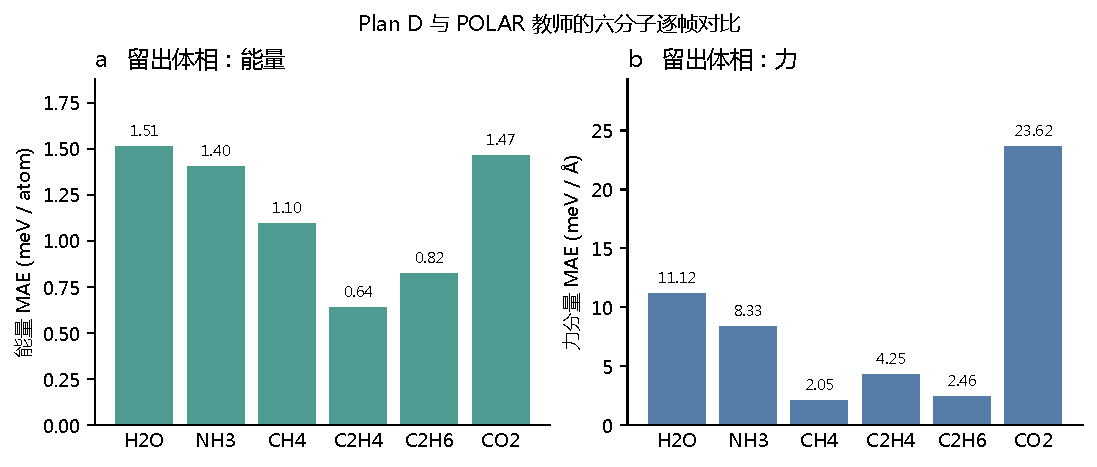
\includegraphics[width=.97\textwidth]{03_six_molecule_student_errors.pdf}
\caption{Plan D 相对 POLAR 教师的留出体相逐帧误差，按分子分组。数值从归档的 \texttt{teacher\_student\_by\_species.json} 读取；这不是相对 DFT 或实验的误差。}\end{figure}

\subsection{数据规模及已发现的限制}
源仓 2026-10-25 的重建记录报告 26,841 个已保留构型，其中 23,376 训练、3465 验证；每种分子的体相帧数为 H$_2$O 4998、NH$_3$ 4574、CH$_4$ 4065、C$_2$H$_4$ 3432、C$_2$H$_6$ 3126、CO$_2$ 4480，气相每种361帧［4］。这些是 E/F 蒸馏构型，并非 26,841 个独立 $c_1/c_2$ 标签。仓库内 \texttt{data/split\_manifest.json} 是较早的 15,641 帧快照，与后来的重建报告不同；新清单和大数据文件能否获取须另行核验。

同一审计记录指出，部分早期状态只有 $0.6\,\mathrm{ps}$、每 $6\,\mathrm{fs}$ 存一帧；平衡、相关性、重复种子及小盒尺寸需要重查［5］。不把这些帧数直接换算为有效独立样本，也不以训练／验证误差替代对目标物理性质的验证。

\subsection{一条水轨迹的权重与质心密度}
OFF23 用 $NVT$ 在 300 K、384 水分子、1 fs 时间步运行，已有 500 ps 生产轨迹；501 个时刻重新计算 OFF23/POLAR 整盒能量。全部501帧的经验权重 ESS 为 2.35，最大单帧权重 59.6\%；图3(a)显示实际权重。删除生产前20帧后仍为约1.20，但这20 ps是基于现有分块现象选出的敏感性切点，不是平衡的证明。OFF 引擎与重算能量去常数后标准差约 $0.030\,\mathrm{eV}$，粒子坐标和日志精度、邻居表与精度路径尚待核对。

图3(b)给出同一批帧的水质心密度：OFF23 等权、POLAR 目标重加权估计及其平滑版。平滑缩小了前后半段差异，但会改变空间分辨率，不能由此断定更准确。条件能量差近似在稀疏区产生超出已有帧支持的峰，故尚不能替代目标参考。$z$ 向分层且质心对统计在 6--8 Å 均值约1.56，不能直接对其套用均匀体相标量 OZ。
\begin{figure}[htbp]\centering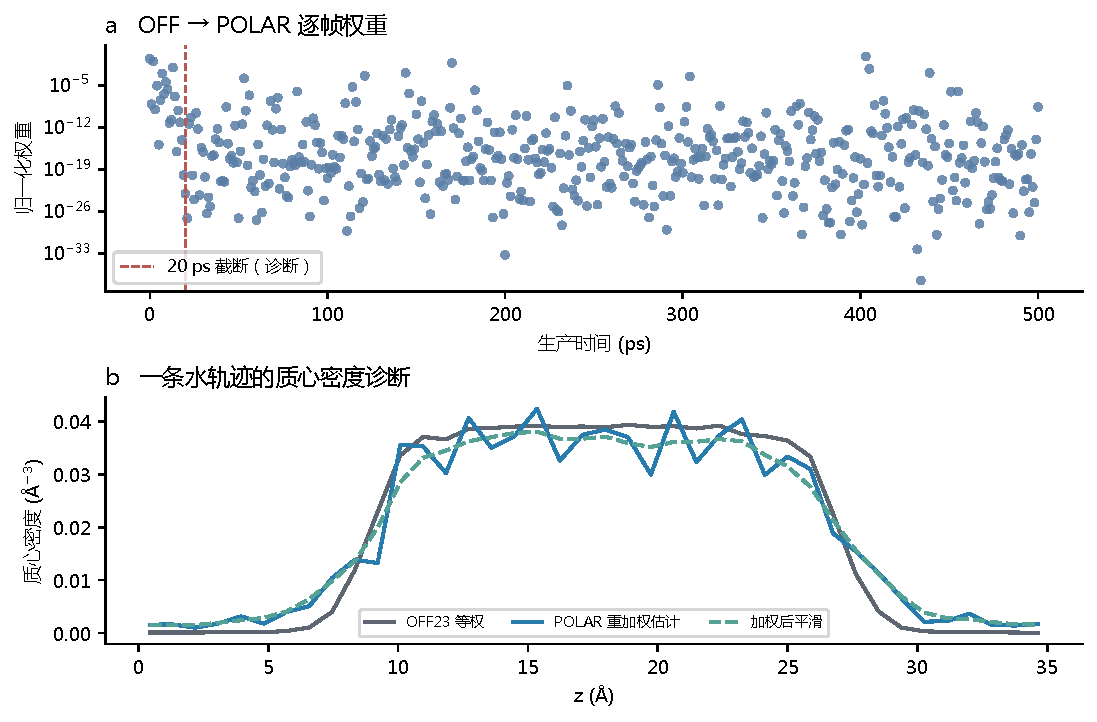
\includegraphics[width=.96\textwidth]{04_water_reweighting_diagnostic.pdf}
\caption{同一条水轨迹的权重和质心密度诊断。加权曲线是目标估计，没有独立 POLAR 密度真值；虚线仅表示后处理平滑。}\end{figure}

\textbf{避免跨仓误读。} \texttt{symmetrix-polar} 的某些旧页面把 OFF23 帧上计算的 $U_{\rm POLAR}-U_{\rm student}$ 评分称为生产尺寸学生自采样 ESS，并据此判定失败；但这501帧来自 OFF23，不是学生势。该分母不匹配采样分布；此数只能作为评分集中度，不能判定学生自采样的重叠。已有 $50\,\mathrm{ps}$ 学生自采样试验可作为独立的小规模线索，但其单轨迹、平衡和相关性不足以证明生产质量。不可把旧页绝对结论搬到本报告。

\section{单体系采样流程与估计器}
图4给出从体系定义到独立物性对照的顺序。对密度格 $k$，当前每帧可用的质心计数写为
\begin{equation}
A_k^{\rho}(x)=\frac{N_k^{\rm COM}(x)}{V_k},\qquad
\widehat{\rho}_{H,k}=\frac{\sum_iq_iA_k^{\rho}(x_i)}{\sum_iq_i}.
\end{equation}
对体相关联，$A_k^g$ 由每帧落在距离壳层内的无序质心对数除以匹配的均匀参考对数。二者分别提供一体密度与两体统计；改变 $A$ 不改变同一组 $q$ 的 Kish ESS。均匀参考、分子身份、有限 $N$、周期边界和力的定义都应保存到数据接口。

后续可比较原始计数、目标力辅助密度、谱函数关联统计与不同频率的 $q$ / $qA$ 估计，评价指标为误差、覆盖、相关时间与 GPU 调用成本。当前文件不包含逐原子 POLAR 力，尚未实施目标力估计。已有 qA 分子每5帧抽样敏感性试验在这条轨迹上高度依赖抽帧起点，不能推广为任何更长采样都失败。
\begin{figure}[htbp]\centering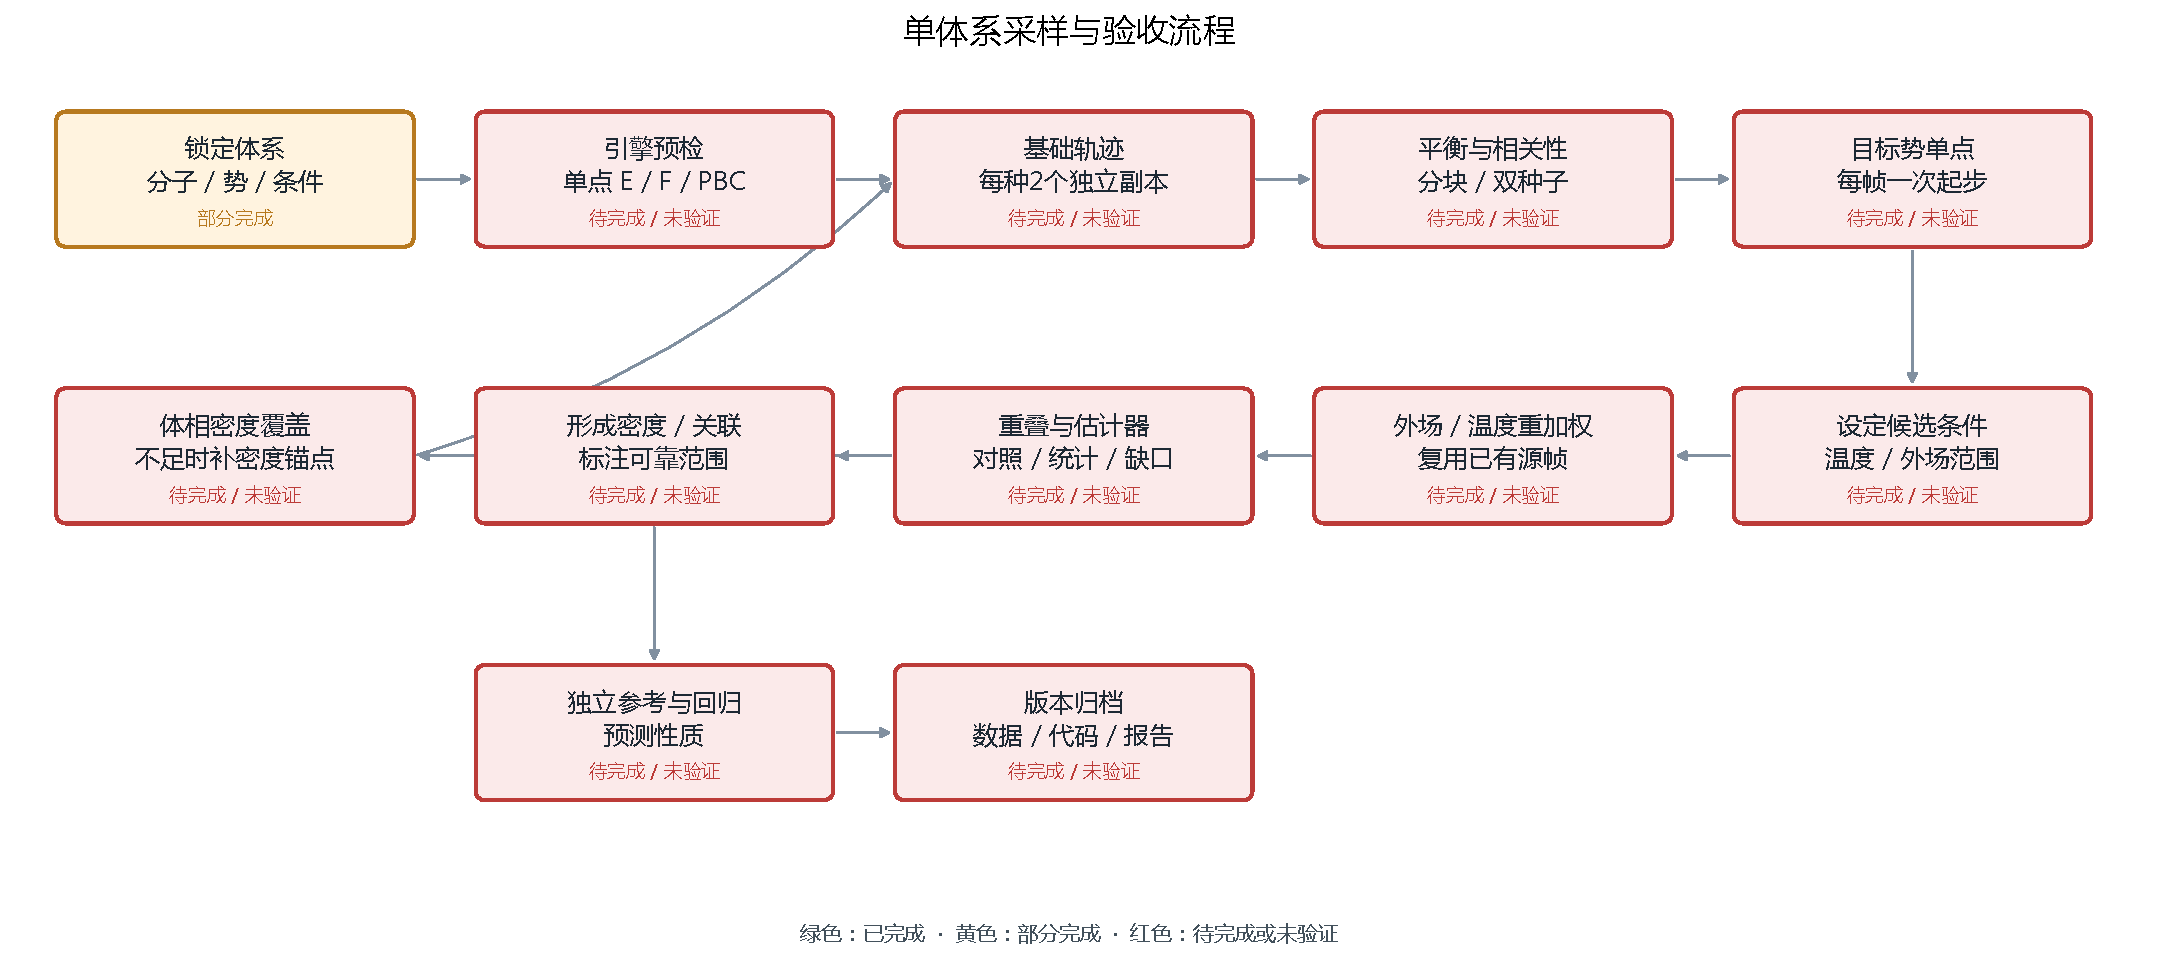
\includegraphics[width=\textwidth]{02_sampling_flow.pdf}
\caption{单体系的计划采样、质量检查和结果归档。红色节点均为后续工作，箭头表示数据流，箭头不表示结果已通过。}\end{figure}

\section{六分子采样预算：基础轨迹复用优先}
\subsection{预算规则与物理前提}
用户希望在可复用的温度和外场范围内，对同一条源轨迹通过重加权生成不同条件的候选统计量。因此预算\textbf{不按每个温度或外场重新增加MD轨迹}。对每帧保存的 OFF23 与 POLAR 基础能量，若目标外势可表示为独立的逐帧外场能，便可后处理不同温度和场强；同一帧的目标能量不必因每个后处理温度重复算。

不过，$2$ 倍权重指数波动线只是当前水样本的对照条件，不能证明密度、$g$ 或 $c_1/c_2$ 的预测误差达到要求。已有水轨迹去除前20帧后的目标权重 ESS 约 1.20，没有独立 POLAR 长轨迹；因此应把它作为\emph{候选扫描范围}，不是六分子无条件复用的验收范围。POLAR 的自洽电荷与极化若随外场变化，目标能量是 $U_H(x;V)$，必须核验并可能对每个场重新评估；简单叠加固定偶极场不是全极化结果。

固定 $N,V$ 的单条 NVT 轨迹总粒子数和平均密度固定；重加权不同外场可以改形状，但不能自动创造不同平均密度的均匀体相样本。已有一条水 500 ps 轨迹呈分层，且 \texttt{test} 仓库没有对应可直接续跑的完整 restart；它先按诊断数据保留，是否能作为所需体相锚点和续跑起点需核实。

\subsection{对照三篇论文：还需要补多少}
为避免把生成剖面数当作独立轨迹数，先把论文给出的样本单元与本项目的候选方案分开：
\begin{center}\small\begin{tabular}{p{2.1cm}p{4.3cm}p{4.1cm}p{3.3cm}}\toprule
方法 & 原文数据单元 & 若机械对齐六分子 & 当前条件 \\\midrule
PNAS & 每流体/势500--1000个随机场MD模拟；每个至少1 ns生产 & 3000--6000个场条件剖面的数量级 & 可先尝试同一基础轨迹重加权生成候选；彼此相关，不能算作3000条独立MD \\
PRL & LJ体相800组密度与$g/c_2$训练数据 & 若每种分子都要求800个体相密度，则为4800组 & 单个NVT基础盒只有一个平均密度；3密度/种只有18组候选，尚未认证 \\
JCTC & 超临界CO$_2$位置--取向密度；SI描述320组剖面 & 若按每种320组的示例估算，则1920组 & 当前非线性分子的取向、统计和模型误差未验收，不能认定已有1920组合格标签 \\\bottomrule
\end{tabular}\end{center}
上表中的3000--6000、4800和1920是将论文单体系数量机械相乘得到的\emph{对齐情景}，不是证明每种分子必须达到的数量。当前本周两个仓库没有给出六种分子合格的目标$c_1/c_2$状态清单，不能从原始帧数精确扣除已有标签；因此无法声称“还差多少个合格标签”。通过重加权生成多个温度或外场剖面可减少额外MD，但准确性和状态覆盖必须逐条件测试，且共用轨迹带来统计相关。

在300 K、无附加场的水例上，保留481帧时 $\operatorname{sd}(\ln q)\simeq13.224$；已有的 $260$ K、$0.25\,\mathrm{V}/\text{\AA}$ 是固定偶极代理在同一源轨迹上的后处理，整体波动约原来的2.106倍。该比较线不包含完整POLAR自洽极化、未给出密度误差，且不能直接外推至其他分子。即使满足这条线，也不能因此认定独立参考验证已完成。

以来源温度 $T_0=300\,\mathrm{K}$ 计算目标温度 $T$ 和目标附加外场时，
\begin{equation}
\ln q(x)=\beta_0 U_L(x)-\beta_T[U_H(x)+U_{\rm ext}(x)]+C.
\end{equation}
$C$ 是构型无关的常数；不能只把源轨迹的 $\beta_0$ 换成 $\beta_T$ 而遗漏源温度项。若同温源和目标有相同外场则该场在能量差中抵消。累计有多少个不同候选场/温度只决定后处理的工作量，不自动决定所需的独立源轨迹数量。

\subsection{最低探索：6条基础轨迹}
如果每种分子暂只设一个基础状态、一个副本，理论上只需6条源势轨迹；每条在充分平衡后以约 $1\,\mathrm{ns}$ 为首轮生产目标。若已有水轨迹与目标状态完全匹配且能可靠续跑，则是其余5种各1条新轨迹加水轨迹延长；当前水数据不满足这个假设的证据，因此不能预先把它抵扣为完整体相1 ns。单轨迹仅供筛查，不能估计独立副本之间的重现性。

\subsection{建议基础批：12条基础轨迹}
为衡量统计重复性，每种分子选择一个适用的基础密度与300 K、各做2条独立副本。每条预算 $200\,\mathrm{ps}$ 预平衡、$1\,\mathrm{ns}$ 生产；如按每 $1\,\mathrm{ps}$ 保存，则每条约1000原始帧。每种2条、$2.4\,\mathrm{ns}$，六种共12条、$14.4\,\mathrm{ns}$ 和约12,000帧。温度及外场的候选剖面全部先从这些基础轨迹复用，不额外乘以外场数。 现有水轨迹的2倍波动线不等于可复用性认证；对每一候选目标需要检查密度与关联估计误差、重叠和独立参考。

\subsection{目标参考另算：建议6条短对照}
为了判断复用得到的统计量是否接近目标，建议优先为每种分子选一个能进入目标势采样的状态，增加1条独立 POLAR 参考轨迹。若只作初步检查，每条先按0.1 ns平衡加0.2 ns生产记账：6条共1.8 ns。它们属于\textbf{目标参考}，与上述12条源轨迹不是同一条，也不按每个场和温度重复；是否足够仍取决于各物理量的相关时间和精度要求。未计这6条时是12条，建议参考一并实施时为\textbf{12条源轨迹 + 6条目标短对照 = 18条计划轨迹}。具体 POLAR 工时尚未在计划硬件和六分子条件下测速。

\subsection{体相覆盖不足时：36条基础轨迹}
若后续 $g/S\to c_2$ 与统一泛函需要每种3个独立平均密度锚点，每个锚点2个独立副本，则每种6条基础轨迹、$7.2\,\mathrm{ns}$、约6000个原始生产帧；六种为36条、$43.2\,\mathrm{ns}$、约36,000帧。这是可调整的探索预算，不是证明3个密度足以训练泛函的结论。

\begin{center}\small\begin{tabular}{lrrrrrr}\toprule
分子 & 基础状态 & 副本 & 基础轨迹 & 基础/ns & 扩展轨迹 & 扩展/ns \\\midrule
H$_2$O &1&2&2&2.4&6&7.2\\
NH$_3$ &1&2&2&2.4&6&7.2\\
CH$_4$ &1&2&2&2.4&6&7.2\\
C$_2$H$_4$ &1&2&2&2.4&6&7.2\\
C$_2$H$_6$ &1&2&2&2.4&6&7.2\\
CO$_2$ &1&2&2&2.4&6&7.2\\\midrule
合计 &6&--&12&14.4&36&43.2\\\bottomrule\end{tabular}\end{center}

基础／扩展分别对应每分子1／3个基础密度，均按每状态2副本；各条时长是0.2 ns预平衡加1 ns生产。对不同温度和外场生成的再加权曲线，它们来自相同帧、彼此统计相关；500条曲线不是500条独立轨迹。训练与验证应按源轨迹、密度、分子和外场分组，避免把共享构型泄漏到训练和测试两侧。

\subsection{目标单点次数与并行资源}
每个用于重加权的时刻要有同一构型的目标能量：若12条基础轨迹每条1000帧都评分，需要约12,000次目标单点；若36条扩展轨迹全部评分，需要约36,000次。每条只评分100帧则分别为1200或3600次，但重加权只能使用已评分的那100帧。不同温度如果势函数本身不随温度改变，可以复用相同帧的基础能量；场依赖自洽极化与力辅助估计则可能需要新增目标场能或力计算，不能将其成本设为零。

真实速度参考仅有 OFF23、1152原子水、Symmetrix/LAMMPS、FP32、1 fs：生产日志500,000步耗时68,990.2 s，即 $7.247$ 步/s 或 $38.33$ GPU时/ns［6］；日志未能确认GPU型号。\textbf{仅作预算情景：}假设六种分子每步都与这个水例一样快，12条基础轨迹约 $14.4\times38.33=552$ GPU时、三卡理想并行约7.7天；36条扩展约 $43.2\times38.33=1656$ GPU时、三卡约23.0天。该假设没有测过其他分子、盒子和势，未含目标单点、等待或重试；真正预算必须按每种分子和实际硬件短跑计时后替换。

如果温度或外场的目标分布缺乏重叠、独立参考不符或统计误差超出事先设定的用途容差，针对这些\emph{失败条件}增加源势、目标势或中间态轨迹；不预先对每一个网格点重复跑。每个分子的状态、势、误差门槛和评估结果都要保存，不应把水的“2倍波动范围”推广为另外五种分子的已验证范围。

\section{数据验收与后续执行顺序}
\begin{enumerate}
\item 核验 OFF23 引擎/重算同帧能量与力、邻居表、目标势模型哈希和长程配置；维持未修前诊断与修正结果的版本对应。
\item 选择每种物质可证明适用的势和阶段一状态；完成独立副本、时间步和盒大小检查，记录真实吞吐、失败率与观测量的相关时间。
\item 对均匀体相，检查 $g(r)$ 尾部、$S(k)$ 低波数与有限尺寸；对不均匀体系保存位置依赖密度/关联，不直接套均匀 OZ。
\item 从随机场密度建立 PNAS 形式的潜变量 $c_1$ 数据，从均匀体相 $g/S$ 构建适用的 $c_2$ 监督；留出场形和状态。
\item 再评估包含分子信息 $\xi$ 的统一模型，分别做留状态、留外场、留分子实验，并用独立参考比较密度、$g(r)$、$S(k)$、相平衡与 cDFT 迭代。新分子没有训练标签时，泛化只能由留分子实验验证。
\end{enumerate}

\section{归档与复现入口}
交互文件 \texttt{workbench/index.html} 离线打开，点击节点查看说明，拖动和修改后导出 JSON。静态流程的 PDF/SVG/PNG 及 Python 源码在 \texttt{figures/}；预算和结果 CSV/JSON、证据哈希及原始仓库路径在归档目录。生成的分子封面图是概念示意，不代表六分子混合体系已被模拟。

\begin{thebibliography}{9}
\bibitem{pnas} A. T. Bui and S. J. Cox, A unified machine-learning framework for ab initio multiscale modeling of liquids, PNAS 123, e2610049123 (2026). \href{https://doi.org/10.1073/pnas.2610049123}{10.1073/pnas.2610049123}.
\bibitem{prl} J. Dijkman et al., Learning Neural Free-Energy Functionals with Pair-Correlation Matching, PRL 134, 056103 (2025). \href{https://doi.org/10.1103/PhysRevLett.134.056103}{10.1103/PhysRevLett.134.056103}.
\bibitem{smoke} Symmetrix-Polar, \textit{Path B six-molecule teacher smoke}, 2026-10-22, source snapshot 68f08d1.
\bibitem{dataset} Symmetrix-Polar, \textit{Bulk + gas dataset rebuild}, 2026-10-25, source snapshot 68f08d1.
\bibitem{audit} Symmetrix-Polar, \textit{Sampling pipeline audit}, 2026-10-23, source snapshot 68f08d1.
\bibitem{log} Test repository, \texttt{log.production\_1fs}, production run at 300 K, source snapshot 65a0423.
\bibitem{jctc} J. Yang et al., High-Dimensional Operator Learning for Molecular Density Functional Theory, JCTC 21, 5905--5915 (2025). \href{https://doi.org/10.1021/acs.jctc.5c00484}{10.1021/acs.jctc.5c00484}; SI, Sec. S1.
\end{thebibliography}
\end{document}
